% !TEX TS-program = XeLaTeX
% use the following command:
% all document files must be coded in UTF-8
\documentclass[portuguese]{textolivre}
% build HTML with: make4ht -e build.lua -c textolivre.cfg -x -u article "fn-in,svg,pic-align"

\journalname{Texto Livre}
\thevolume{15}
%\thenumber{1} % old template
\theyear{2022}
\receiveddate{\DTMdisplaydate{2021}{11}{30}{-1}} % YYYY MM DD
\accepteddate{\DTMdisplaydate{2021}{12}{2}{-1}}
\publisheddate{\DTMdisplaydate{2022}{2}{16}{-1}}
\corrauthor{Bruna de Almeida Oliveira Moreira}
\articledoi{10.35699/1983-3652.2022.37306}
%\articleid{NNNN} % if the article ID is not the last 5 numbers of its DOI, provide it using \articleid{} commmand
% list of available sesscions in the journal: articles, dossier, reports, essays, reviews, interviews
\articlesessionname{articles}
\runningauthor{Moreira e Espírito Santo} 
%\editorname{Leonardo Araújo} % old template
\sectioneditorname{Bárbara Amaral da Silva}
\layouteditorname{Daniervelin Pereira}

\title{“Essa é nova! Gringo quer nos ensinar a falar a nossa própria língua”: ideologias linguísticas e posicionamentos identitários em uma página do Facebook}
\othertitle{“That’s news to me! Gringo wants to teach us how to speak our own language”: language ideologies and identity positioning on a Facebook page}
% if there is a third language title, add here:
%\othertitle{Artikelvorlage zur Einreichung beim Texto Livre Journal}

\author[1]{Bruna de Almeida Oliveira Moreira \orcid{0000-0001-8549-4844} \thanks{Email: \url{brunaalmeida.ufrb@gmail.com}}}
\author[1]{Diogo Oliveira do Espírito Santo \orcid{0000-0003-4805-4430} \thanks{Email: \url{diogo.oliveira@ufrb.edu.br}}}
\affil[1]{Universidade Federal do Recôncavo da Bahia, Centro de Formação de Professores, Amargosa, BA, Brasil.}

\addbibresource{article.bib}
% use biber instead of bibtex
% $ biber article

% used to create dummy text for the template file
\definecolor{dark-gray}{gray}{0.35} % color used to display dummy texts
\usepackage{lipsum}
\SetLipsumParListSurrounders{\colorlet{oldcolor}{.}\color{dark-gray}}{\color{oldcolor}}

% used here only to provide the XeLaTeX and BibTeX logos
\usepackage{hologo}

% if you use multirows in a table, include the multirow package
\usepackage{multirow}

% provides sidewaysfigure environment
\usepackage{rotating}

% CUSTOM EPIGRAPH - BEGIN 
%%% https://tex.stackexchange.com/questions/193178/specific-epigraph-style
\usepackage{epigraph}
\renewcommand\textflush{flushright}
\makeatletter
\newlength\epitextskip
\pretocmd{\@epitext}{\em}{}{}
\apptocmd{\@epitext}{\em}{}{}
\patchcmd{\epigraph}{\@epitext{#1}\\}{\@epitext{#1}\\[\epitextskip]}{}{}
\makeatother
\setlength\epigraphrule{0pt}
\setlength\epitextskip{0.5ex}
\setlength\epigraphwidth{.7\textwidth}
% CUSTOM EPIGRAPH - END

% LANGUAGE - BEGIN
% ARABIC
% for languages that use special fonts, you must provide the typeface that will be used
% \setotherlanguage{arabic}
% \newfontfamily\arabicfont[Script=Arabic]{Amiri}
% \newfontfamily\arabicfontsf[Script=Arabic]{Amiri}
% \newfontfamily\arabicfonttt[Script=Arabic]{Amiri}
%
% in the article, to add arabic text use: \textlang{arabic}{ ... }
%
% RUSSIAN
% for russian text we also need to define fonts with support for Cyrillic script
% \usepackage{fontspec}
% \setotherlanguage{russian}
% \newfontfamily\cyrillicfont{Times New Roman}
% \newfontfamily\cyrillicfontsf{Times New Roman}[Script=Cyrillic]
% \newfontfamily\cyrillicfonttt{Times New Roman}[Script=Cyrillic]
%
% in the text use \begin{russian} ... \end{russian}
% LANGUAGE - END

% EMOJIS - BEGIN
% to use emoticons in your manuscript
% https://stackoverflow.com/questions/190145/how-to-insert-emoticons-in-latex/57076064
% using font Symbola, which has full support
% the font may be downloaded at:
% https://dn-works.com/ufas/
% add to preamble:
% \newfontfamily\Symbola{Symbola}
% in the text use:
% {\Symbola }
% EMOJIS - END

% LABEL REFERENCE TO DESCRIPTIVE LIST - BEGIN
% reference itens in a descriptive list using their labels instead of numbers
% insert the code below in the preambule:
%\makeatletter
%\let\orgdescriptionlabel\descriptionlabel
%\renewcommand*{\descriptionlabel}[1]{%
%  \let\orglabel\label
%  \let\label\@gobble
%  \phantomsection
%  \edef\@currentlabel{#1\unskip}%
%  \let\label\orglabel
%  \orgdescriptionlabel{#1}%
%}
%\makeatother
%
% in your document, use as illustraded here:
%\begin{description}
%  \item[first\label{itm1}] this is only an example;
%  % ...  add more items
%\end{description}
% LABEL REFERENCE TO DESCRIPTIVE LIST - END


% add line numbers for submission
%\usepackage{lineno}
%\linenumbers

\begin{document}
\maketitle

\begin{polyabstract}
\begin{abstract}
Neste artigo, nosso objetivo é investigar posicionamentos identitários negociados entre usuários de plataformas de redes sociais. Voltamo-nos, assim, para práticas comunicativas desenvolvidas na página do Facebook Greengo Dictionary, para analisar e discutir postagens e comentários por meio de um estudo qualitativo centrado no discurso online. Para esse fim, nos baseamos nos conceitos de comunidade virtual \cite{recuero_comunidades_2009}, comunidade discursiva \cite{swales_repensando_1992,araujo_comunidade_2020}, posturas \cite{barton_linguagem_2015}, posicionamentos \cite{harre_positioning_1999} e táticas de intersubjetividade \cite{bucholtz_language_2004,bucholtz_identity_2005}, que nos permitiram compreender a construção discursiva dos posicionamentos identitários e as ideologias linguísticas \cite{moita_lopes_ingles_2008,moita_lopes_ideologia_2013} que orientam os diferentes usos de inglês e português online. Neste artigo, apontamos, por fim, que, ao se engajarem em práticas de linguagem fluidas e híbridas, os usuários do Facebook se posicionam frente a uma gama de propósitos comunicativos, acentuando não só a criatividade e humor que caracterizam a página Greengo Dictionary, mas também discursos normativistas que atuam para o estabelecimento de diferentes relações identitárias.

\keywords{Ideologia linguística \sep Posicionamentos identitários \sep Facebook}
\end{abstract}

\begin{english}
\begin{abstract}
In this article, we aim to investigate identity positionings negotiated between social media users. We rely on communicative practices on a Facebook page, “Greengo Dictionary”, to analyze and discuss posts and comments through a discourse-centered online qualitative study. To this end, we draw on the notions of virtual community \cite{recuero_comunidades_2009}, discourse community \cite{swales_repensando_1992,araujo_comunidade_2020}, stances \cite{barton_linguagem_2015}, positioning \cite{harre_positioning_1999}, and tactics of intersubjectivity \cite{bucholtz_language_2004,bucholtz_identity_2005}, which provided us with opportunities to understand the discursive construction of identity positioning and the language ideologies underlying the use of English and Portuguese online. In conclusion, we observe that while engaging in fluid and hybrid language practices, Facebook users position themselves in relation to a wide range of communicative purposes, which highlight not only the creativity and humor that characterize the Greengo Dictionary page, but also the linguistic normativism that contributes to the development of different identity relations.

\keywords{Language ideology \sep Identity positioning \sep Facebook}
\end{abstract}
\end{english}
% if there is another abstract, insert it here using the same scheme
\end{polyabstract}

\section{Introdução}\label{sec-intro}
Vivemos em um mundo cada vez mais conectado, o que nos permite não só realizar diversas atividades, mas ter acesso a uma variada gama de recursos tecnológicos. Nesse contexto, o uso de plataformas e mídias digitais têm oportunizado novas formas de interação e intensificado o engajamento em diferentes grupos de afinidade \cite{leppanen_multilingualism_2012}, com sujeitos negociando sentidos e se posicionando frente ao que é publicizado pelos seus pares. Tais práticas vêm chamando a atenção de pesquisadores de diferentes campos do conhecimento, principalmente no âmbito dos estudos da linguagem, interessados nos processos de construção de sentido em sites de redes sociais, como o Facebook \cite{bolander_constructing_2010,bolander_peter_2015,lee_micro-blogging_2011,bolander2017,dovchin_language_2020}. Dessa maneira, torna-se necessário refletir sobre o que entendemos por língua e identidade, considerando os variados recursos multimodais com os quais os sujeitos agem uns em relação aos outros.

Apresentadas as prerrogativas, este artigo tem como objetivo analisar posicionamentos identitários e ideologias linguísticas negociadas em uma página do Facebook. Trata-se de uma pesquisa qualitativa centrada no discurso online \cite{barton_linguagem_2015}, cujos dados foram gerados a partir da coleta de comentários e postagens da página Greengo Dictionary, em que sujeitos avaliam diferentes discursos relacionados às línguas inglesa e portuguesa. Embasar-nos-emos nos conceitos de comunidade virtual \cite{recuero_comunidades_2003,recuero_comunidades_2009} e comunidades discursivas \cite{swales_repensando_1992,araujo_comunidade_2020}, a fim de investigarmos os espaços em que os sujeitos interagem a partir de uma rede de recursos verbais e não verbais, e propomos pensar as línguas desde uma perspectiva de fronteira, hibridação e trânsito \cite{moita_lopes_ingles_2008,moita_lopes_ideologia_2013}.

Complementarmente, no intuito de analisar a construção discursiva de posicionamentos identitários com relação aos diferentes usos linguísticos, bem como  problematizar as maneiras por meio das quais os sujeitos agem uns em relação aos outros, lançaremos mão de pressupostos da Teoria dos Posicionamentos \cite{harre_positioning_1999}, posturas \cite{barton_linguagem_2015} e das táticas de intersubjetividade, proposta de análise da construção discursiva da identidade desenvolvida por \textcite{bucholtz_language_2004,bucholtz_identity_2005}. Ademais, problematizaremos, à luz dos conceitos de ideologia linguística \cite{moita_lopes_ingles_2008,moita_lopes_ideologia_2013} e metalinguagem ou discurso metalinguístico \cite{barton_linguagem_2015}, como as práticas de linguagem na página Greengo Dictionary indicam posições ideológicas que se movimentam por normas e expectativas diversas, ressaltando a intrínseca relação entre discursos \textit{on} e \textit{offline}.

\section{Pressupostos teóricos}\label{sec-normas}
Para compreendermos as práticas de linguagem de sujeitos que se engajam em plataformas de redes sociais, devemos conhecer os meios pelos quais os discursos são negociados\footnote{Entendemos aqui discurso como a construção social do sentido, isto é, uma forma de ação no mundo. Alinhados a \textcite{moita_lopes_identidades_2002}, defendemos, portanto, que investigar os processos discursivos significa se envolver na análise de como os sujeitos constroem sentido de suas práticas por meio da linguagem.}. Diante disso, a página Greengo Dictionary será aqui entendida em termos de comunidade virtual e de comunidade discursiva \cite{swales_repensando_1992,araujo_comunidade_2020}. Segundo tais perspectivas, os sujeitos negociam suas práticas discursivas através da intercomunicação, envolvendo a participação e o \textit{feedback} constante de seus pares, por meio da apropriação de gêneros discursivos para alçarem propósitos comunicativos diversos. Entendemos, assim, comunidade virtual como “[...] um conjunto de atores e suas relações que, através da interação social em um determinado espaço constitui laços e capital social”. \cite[p. 144]{recuero_comunidades_2009}. Dessa forma, os usuários constituem grupos em que a interação e os laços sociais são preponderantes para a negociação de sentido mediado pela tecnologia digital.	Quanto à comunidade discursiva \cite{swales_repensando_1992,rampazzo_revisitar_2019,araujo_comunidade_2020}, podemos defini-la como o ambiente em que os indivíduos se unem com um propósito comunicativo específico. Por isso, elas constituem:

\begin{quote}
    [...] um grupo sócio-retórico heterogêneo que compartilha objetivos e interesses ocupacionais ou recreativos, distinguindo-se de comunidade de fala, definida como um grupo sociolinguístico homogêneo de pessoas que compartilham região geográfica e background. \cite[p. 08]{swales_repensando_1992}\footnote{Toda tradução de textos em língua estrangeira é de nossa responsabilidade.}.
\end{quote}

Isso posto, é nas interações nessas comunidades que diferentes práticas de linguagem são construídas, e é por meio delas que os sujeitos ocupam e atribuem diferentes posições discursivas frente ao que é publicizado. No caso deste artigo, estamos nos referindo aos posicionamentos frente ao que entendemos por língua inglesa e portuguesa.

Compreenderemos as práticas linguísticas que envolvem o inglês e o português a partir das propostas de \textcite{moita_lopes_ingles_2008,moita_lopes_ideologia_2013}. O pesquisador discute tais línguas a partir de um viés de hibridismo e desterritorialização, isto é, como recursos que os sujeitos empregam em suas interações, permitindo que transitem entre diferentes semioses e discursos para alcançar seus propósitos comunicativos. A partir dessa orientação, se deixa de lado a concepção de uma língua considerada “pura” e “certa”, conforme a estabelecida pela gramática normativa \cite{bezerra_normativismo_2016}, em que se impõe um único “padrão” às práticas de linguagem. O foco, assim, se desloca do sistema linguístico stricto sensu para as estratégias de negociação que os sujeitos empregam, constituindo “[...] de modo situado, em meio a conflitos e assimetrias, ‘uma forma hibrida’ de comunicação, que mistura diferentes línguas e linguagens, ao mesmo tempo em que sinaliza subjetividades e identidades”. \cite[p. 430]{rocha_ensino_2015}.							

Deslocar-se da ideia de purismo para a de hibridismo e de práticas transfronteiriças nos guia a uma abordagem que ressalta os usos criativos da língua(gem). Nessa direção, \textcite{moita_lopes_ideologia_2013} %Moita Lopes (2013) 
esclarece que o mais importante no processo investigativo dessas práticas é discutir que ideologias estão em operação quando os sujeitos agem por entre línguas, linguagens e identidades, se apropriando de diferentes discursos e recursos comunicativos. O autor conclui que, em um mundo constituído por fluxos de textos e pessoas, é necessário reteorizar o que entendemos por língua, com vistas à construção de novas perspectivas, afastando-a, assim, de uma ideologia linguística da norma.

Outras perspectivas que problematizam a noção de uma língua “correta” são aquelas das ideologias linguísticas de \textcite{moita_lopes_ingles_2008,moita_lopes_ideologia_2013}, que englobam o debate sobre as crenças, definições, teorias e compreensões de como uma língua(gem) deve ou não ser utilizada, e as de \textcite{barton_linguagem_2015}, centradas no conceito de metalinguagem. Face ao exposto, neste artigo, nos embasamos em ambos os conceitos por oferecerem caminhos produtivos para a investigação dos discursos que os sujeitos constroem sobre a língua(gem) em diferentes espaços de interação. 					
\textcite[p. 22]{moita_lopes_ideologia_2013}, se embasando em \textcite[p. 3]{woolard_introduction:_2008}, explica ideologia linguística como:

\begin{quote}
    [...] as compreensões, ‘tanto explícitas quanto implícitas que traduzem a interseção da linguagem e os seres humanos em um mundo social’ [...] ou compreensões de como a linguagem ou línguas específicas têm sido ou são entendidas com base em como são situadas em certas práticas sócio-históricas, inclusive aquelas visões elaboradas por pesquisadores e teóricos da linguagem, derivadas do espírito intelectual ou da perspectiva epistemológica de seu tempo.
\end{quote}

Já \textcite[p. 144]{barton_linguagem_2015}, interessados na comunicação digital, definem metalinguagem como “[...] enunciados que expressam crenças e atitudes sobre a linguagem”. Tais perspectivas voltadas para a língua(gem) (e as práticas sociais delas decorrentes) se desenvolvem por meio do discurso metalinguístico, expresso de diversas formas e por recursos variados. Aqui, nos interessa o discurso metalinguístico que indexa “[...] um importante tipo de visão de linguística popular observada \textit{online} [...] quando as pessoas falam sobre o que elas julgam ser bom ou ruim”. \cite[p. 147]{barton_linguagem_2015}. Em síntese, o discurso metalinguístico se refere não só ao que os sujeitos consideram como certo e esperado, mas também às posições ideológicas negociadas em diferentes configurações espaço-temporais, sejam elas \textit{on} ou \textit{offline}. 

As ideologias que embasam o uso de línguas por participantes da comunidade virtual/discursiva Greengo Dictionary são expressas a partir do que podemos chamar de posicionamento, conceito teórico e metodológico central na Teoria dos Posicionamentos \cite{harre_positioning_1999} e na noção de posturas \cite{barton_linguagem_2015}.										

A Teoria dos Posicionamentos é um esforço multidisciplinar que transita entre perspectivas da psicologia cultural/discursiva, feministas e pós-estruturalistas, com o objetivo de compreender como os sujeitos negociam posições no discurso para performarem determinadas ações sociais. De acordo com \textcite{kayi-aydar_positioning_2019}, a Teoria busca investigar práticas que inibem certos grupos sociais de agirem ou performarem determinados atos de fala em práticas discursivas. 					

\textcite{harre_positioning_1999} definem posicionamento como:

\begin{quote}
    [...] construção discursiva de histórias pessoais que fazem as ações de uma pessoa inteligíveis e relativamente determinadas como atos sociais e dentro dos quais os membros de uma conversa têm locações específicas. \cite[p. 16]{harre_positioning_1999}.
\end{quote}

Nessa mesma direção, \textcite[p. 118]{barton_linguagem_2015} compreendem posturas como o “[...] posicionamento das pessoas em relação a si mesmas, ao que é dito, e a outras pessoas ou objetos”. Dessa forma, é possível inferir que é por meio do ato discursivo que os sujeitos se expressam, e é através dos posicionamentos/posturas que podemos investigar as práticas discursivas mediadas pela tecnologia digital, uma vez que “[...] o posicionamento se tornou um ato discursivo fundamental na interação online”. \cite[p. 118]{barton_linguagem_2015}. 

Fica sugerido, portanto, um diálogo entre essas propostas e a visão bakhtiniana de linguagem, segundo a qual toda compreensão de um enunciado\footnote{Neste artigo, também assumimos uma perspectiva bakhtiniana de enunciado, entendido como uma atividade de linguagem concreta, irrepetível, realizada num determinado espaço e tempo e socio-historicamente situada \cite{molon_o_2012}.} é acompanhada de uma atitude responsiva viva, isto é,

\begin{quote}
    [...] toda compreensão é prenhe de resposta e, de uma forma ou de outra, forçosamente a produz: [...] o ouvinte que recebe e compreende a significação de um discurso adota simultaneamente, para com esse discurso, uma atitude responsiva ativa: ele concorda ou discorda (total ou parcialmente), completa, adapta, apronta-se para executar. \cite[p. 290]{bakhtin_estetica_1992}.
\end{quote}

Essa atitude responsiva, desse modo, caracteriza a tomada de posicionamento dos sujeitos, já que toda resposta a enunciados é sempre marcada por uma atitude valorativa.	

Assim, observamos que a noção de posturas e posicionamentos coloca em voga o entendimento de identidade como construção discursiva, corroborando a afirmação de \textcite[p. 34]{moita_lopes_identidades_2002} de que a identidade está sempre em processo, “[...] pois é dependente da realização discursiva em circunstâncias particulares: os significados que os participantes dão a si mesmos e aos outros engajados no discurso”. Com isso, tal visão de identidade nos permitirá investigar as maneiras a partir das quais os sujeitos se constroem uns em relação aos outros, isto é, como se posicionam com base em quem eles são ou querem ser na interação. Para isso, faz-se necessária uma abordagem adequada ao entendimento de identidade como discurso. Falaremos sobre esse aspecto na próxima seção.

\section{Percurso teórico-metodológico}\label{sec-conduta}
A perspectiva metodológica que orienta este artigo é a da pesquisa qualitativa centrada no discurso \textit{online}, por considerar que “[...] as práticas de produção de texto \textit{online} não implicam apenas analisar características estruturais da língua, mas também observar modos particulares de criação e utilização de textos”. \cite[p. 221]{barton_linguagem_2015}. Logo, nos interessa investigar de quais maneiras os sujeitos usam textos para se posicionarem discursivamente\footnote{Esclarecemos que o estudo aqui proposto está voltado única e exclusivamente para procedimentos de análise textual/discursiva dos posicionamentos identitários emergentes de \textit{posts} de uma página pública do Facebook. Logo, informamos que não houve qualquer contato ou geração de dados pessoais com os sujeitos envolvidos nas postagens.}.

Como já antecipado, a comunidade discursiva que dará base ao nosso estudo é a Greengo Dictionary, uma página do Facebook criada em 8 fevereiro de 2019, sob o nome de Aurelius Dictionary. Atualmente, ela conta com 305.630 seguidores e 283.500 curtidas\footnote{Dados de novembro de 2021.}, sem mencionar os números do Instagram e do Twitter, o que evidencia a sua popularidade e relevância para estudos sobre práticas de linguagem \textit{online}. Segundo informações da própria página \cite{greengo_dictionary_sobre_2021}, seu objetivo é a construção de um espaço em que os usuários podem participar não só enviando traduções ‘bizarras’ de expressões brasileiras em inglês, como também compartilhando memes e publicações de outras plataformas digitais, cujas temáticas estejam dentro do escopo da página. Embora se divulgue que a \textcite{greengo_dictionary_sobre_2021} é para “pura diversão”, e as contribuições dos seus usuários venham acompanhadas de memes bem-humorados, grande parte das postagens apresenta cunho de crítica social e política.

Neste artigo, serão analisadas três publicações\footnote{Dados coletados da página entre os meses de setembro e novembro de 2021.} e seus respectivos comentários realizados por diferentes usuários. Elas foram escolhidas para este estudo por ilustrarem as principais temáticas aqui discutidas, quais sejam, hibridismo, a ideia de língua pura e correta, além de fundamentarem a discussão de uma profusão de posicionamentos identitários e ideologias linguísticas.

Sobre esse último ponto, é necessário esclarecer que os posicionamentos no discurso serão analisados a partir da imbricação de duas propostas teórico-metodológicas: a primeira, aqui já apresentada, é oriunda da Teoria dos Posicionamentos, e a segunda das táticas de intersubjetividade, de \textcite{bucholtz_language_2004,bucholtz_identity_2005}.

No desenvolvimento da Teoria dos Posicionamentos, \textcite{harre_positioning_1999} discutem possibilidades analíticas para a investigação de como os sujeitos atribuem ou reivindicam posições no discurso. Uma delas se centra na discussão dos posicionamentos de primeira, segunda e terceira ordens.

O posicionamento de primeira ordem ocorre quando o ato de se posicionar ou de posicionar alguém não é desafiado: “[...] refere-se à maneira como as pessoas se posicionam e posicionam outras dentro de um espaço essencialmente moral através do uso de variadas categorias identitárias [...]”. \cite[p. 20]{harre_positioning_1999}. No entanto, quando o posicionamento de primeira ordem é desafiado, isto é, não aceito pelos envolvidos na interação, é configurado um caso de posicionamento de segunda ordem. Já o posicionamento de terceira ordem é alcançado quando sujeitos que não participam da interação são posicionados por outros.

A partir dessa proposta, se torna possível investigar o papel dos posicionamentos na constituição identitária dos sujeitos e como esses acatam, desafiam ou subvertem posições atribuídas discursivamente. Neste artigo, além de nos embasarmos nesses pressupostos, os expandiremos no intuito de incluir a perspectiva das táticas de intersubjetividade, como proposta por \textcite{bucholtz_language_2004,bucholtz_identity_2005}.

As táticas de intersubjetividade constituem um quadro analítico desenvolvido com o objetivo de descrever como e por que as identidades são construídas discursivamente. A partir desse quadro, \textcite[p. 586]{bucholtz_identity_2005} propõem pensar as identidades como “[...] fenômenos sociais e relacionais que emergem e circulam em contextos discursivos de interação local, ao invés de uma estrutura estática locada primordialmente na psique individual ou em categorias fixas”. Com tal entendimento, portanto, as autoras reforçam a noção de identidade como o posicionamento de si e do outro, envolvendo desde categorias identitárias macro (como identidades nacionais, sociais e de gênero) até as mais temporárias e interacionalmente alcançadas.

Embasado no que \textcite{bucholtz_language_2004,bucholtz_identity_2005} denominam de linguística sociocultural, o modelo das táticas de intersubjetividade se refere às relações criadas entre os sujeitos na e para a prática identitária, que podem ser resumidas em três pares: adequação/distinção, autenticação/desnaturalização e autorização/ deslegitimação.

A adequação está relacionada à busca de semelhanças sociais, em que as diferenças são deixadas de lado em favor de semelhanças que podem vir a ser relevantes em determinados contextos comunicativos. De acordo com \textcite[p. 599, grifo das autoras]{bucholtz_identity_2005}:

\begin{quote}
    [...] [o] termo \textit{adequação} enfatiza o fato de que para que os grupos ou sujeitos sejam posicionados como iguais, eles não precisam – e em todo caso não podem – ser idênticos, mas devem ser entendidos como suficientemente similares para propósitos interacionais.
\end{quote}

Já a distinção foca na relação identitária de diferenciação, isto é, na supressão das similaridades que podem prejudicar a construção da diferença entre grupos sociais e sujeitos.

No segundo par, a autenticação se refere à relação construída entre sujeitos que reivindicam autenticidade de suas posições identitárias, isto é, buscam performar identidades “genuínas”. Em contrapartida, a relação de desnaturalização, conforme \textcite[p. 451, grifo do autor]{borba_discurso_2009},

\begin{quote}
    [...] refere-se ao processo pelo qual uma identidade é desestabilizada a partir de rupturas percebidas ou construídas em sua \textit{performance}, produzindo-a (1) como insatisfatória para os padrões locais ou (2) como descontínua e fragmentada.
\end{quote}

Por fim, o par autorização/deslegitimação está relacionado à tentativa de legitimar uma identidade (autorização) ou de negá-la (deslegitimação) por meio da autoridade/poder institucional atribuído aos sujeitos.

Faz-se importante pontuar que tal modelo não deve ser entendido como uma proposta exaustiva de análise de posicionamentos identitários, tampouco suas relações devem ser tomadas como mutuamente exclusivas. Pelo contrário, essa é uma tentativa de investigar uma dimensão específica da construção identitária, qual seja, a relacional, com foco nas performances identitárias, construídas discursivamente e que, muitas vezes, se sobrepõem umas às outras.

Com isso em mente, lançamos mão das táticas de intersubjetividade, atrelando-as às noções de postura e posicionamento por considerarmos que tais propostas podem contribuir para investigar as motivações para a negociação identitária de sujeitos que se posicionam \textit{online}. Tal combinação pode oferecer um quadro holístico de análise dos processos através dos quais se atribuem e se negam posições identitárias.

Feitas as considerações metodológicas do nosso trabalho, seguimos para as seções de análise e de discussão dos dados, com base nos pressupostos até aqui discutidos.

\section{Análise dos dados}\label{sec-fmt-manuscrito}
Postagem 1\footnote{Toda informação que pudesse identificar os sujeitos foi ocultada, a fim de assegurar a anonimidade desses.}

\begin{figure}[htbp]
 \centering
 
\includegraphics[width=0.85\textwidth]{Fig1.png}
 \caption{Postagem 1 da Greengo Dictionary.}
 \label{fig1}
 \source{GREENGO DICTIONARY, Facebook \url{https://www.facebook.com/greengodictionary}. Acesso em: 10 de set. de 2021.}
\end{figure}

A postagem em questão (\Cref{fig1}) é um compartilhamento de uma publicação feita por um usuário do Twitter, cuja temática se relaciona com as discussões mais recorrentes na Greengo Dictionary. Observa-se que ela se centra na crítica a uma possível autodepreciação \cite{barton_linguagem_2015} dos brasileiros com relação ao inglês por eles falado. Fazemos essa observação partindo do enunciado “Síndrome de viralata”, que retoma o chamado “complexo de vira-latas” usado pelo dramaturgo brasileiro \textcite{rodrigues_sombra_1993} para caracterizar o estado de inferioridade em que os próprios brasileiros se colocam frente ao que é estrangeiro. Nessa dinâmica, ao passo em que se atribuem uma posição de inferioridade com relação a esse “outro” estrangeiro, os brasileiros o elevam a uma posição hierarquicamente superior.												

Em sua crítica, o Sujeito A ressalta a diferença entre brasileiros e estrangeiros a partir da manipulação de diferentes recursos linguísticos, o que pode ser ilustrado pelo contraste entre os enunciados “seu inglês” e “português todo errado”. O primeiro indica que o inglês falado pelos brasileiros é tão válido quanto qualquer outro, não devendo, portanto, ser motivo de vergonha; em contrapartida, o português falado pelo outro, “o chefe francês que vive no Brasil há 200 anos”, é caracterizado como “todo errado”\footnote{Aqui, fica sugerido que o “chefe francês” seja uma referência a um dos jurados de um famoso programa de culinária no Brasil.}.							

Nesse cenário, percebemos que enquanto busca posicionar os brasileiros como falantes “legítimos” de língua inglesa, o Sujeito A também posiciona o outro (francês) como “ilegítimo”, o que nos leva a considerar tal prática de posicionamento como uma relação de distinção \cite{bucholtz_language_2004,bucholtz_identity_2005}. Sobre isso, \textcite[p. 384]{bucholtz_language_2004} afirmam que:

\begin{quote}
    [...] [a] distinção, frequentemente, opera de modo binário, estabelecendo uma dicotomia entre identidades sociais construídas como opostas ou contrastivas. Assim, ela tende a reduzir a complexa variabilidade social a uma única dimensão: nós versus eles.
\end{quote}

Com isso, é possível inferir que os efeitos de sentido produzidos pela e na postagem são alcançados através da relação de distinção que se estabelece entre os brasileiros (nós) e o estrangeiro (ele). Isso porque a partir dessa publicação, o Sujeito A não só critica um complexo de inferioridade por parte dos brasileiros, com vistas à valorização do inglês falado por eles, mas também se autoposiciona como aquele que teria a autoridade para julgar o português do “outro” como ilegítimo.	

Orientado pela relação de deslegitimação, que é alcançada pela sua posição frente ao português “todo errado” do “chefe francês”, o Sujeito A dá pistas de um possível alinhamento a uma ideologia linguística da norma, ou como \textcite{bagno_inevitavel_2002} denomina “norma-padrão”. Segundo o autor, tal ideologia linguística é orientada por uma idealização nebulosa de correção linguística e traduz uma concepção abstrata de língua, em que essa “[...] é pensada como se não estivesse neste mundo, como se fosse um objeto místico a ser buscado sem jamais poder ser alcançado”. \cite[p. 22]{bagno_inevitavel_2002}.									

Complementarmente, \textcite[p. 23]{moita_lopes_ideologia_2013}, se embasando em \textcite[p. 501]{kroskrity_language_2004}, nos diz que tal norma, embasada em um normativismo linguístico “[...] desampara sociolinguisticamente aqueles que não dominam a língua considerada legítima”. Isso reforça a nossa consideração de que para o Sujeito A, todos que moram no Brasil “há mais de 200 anos” deveriam falar um português “correto”. O que se observa, portanto, é uma complexa e contraditória relação de posicionamentos identitários orientada pela ideologia linguística da norma que serve tanto para valorizar o que é nacional (leia-se o “inglês brasileiro”), como para deslegitimar práticas linguísticas estrangeiras. Logo, ao (des)autenticar o uso de línguas por diferentes sujeitos em sua publicação, o Sujeito A acaba indexando suas próprias identidades linguísticas e negociando diferentes posições discursivas, tais como a de sujeito com poder para validar usos linguísticos e a de falante legítimo de diferentes línguas.										
Outras relações identitárias também podem ser observadas na seção de comentários da postagem em questão, como mostramos na sequência (\Cref{fig2}).

\begin{figure}[htbp]
 \centering
 
\includegraphics[width=0.75\textwidth]{Fig2.png}
 \caption{Seção de comentários 1 da Greengo Dictionary.}
 \label{fig2}
 \source{GREENGO DICTIONARY, Facebook \url{https://www.facebook.com/greengodictionary}. Acesso em: 10 de set. de 2021.}
\end{figure}

Nesses comentários, são retomados os posicionamentos com relação à ideologia linguística da norma. Embora não se possa mensurar o que tais sujeitos entendem por inglês “correto” ou “errado”, sugerimos que esse esteja sendo compreendido em termos de “inglês padrão” \cite{stubbs_lingua_2002}.

Segundo \textcite{stubbs_lingua_2002}, falar corretamente o inglês está além de uma avaliação puramente descritiva do seu sistema linguístico. Para esse autor, “[...] [f]alar ‘corretamente’ é, no mais das vezes, tomado \textit{em si mesmo} como prova de alguém bem-educado”. \cite[p. 105, grifos do autor]{stubbs_lingua_2002}. Logo, a hostilização frente ao inglês “errado” é orientada muito mais por uma ideologia linguística da prescrição, embasada em classe social e no prestígio de uma cultura particular, do que pelas normas gramaticais que regem essa língua.

A partir desses comentários, é possível observar também que as relações de intersubjetividade são apresentadas como uma estratégia de resistência à tal prescrição. Fazemos essa ponderação com base em posicionamentos que desafiam à possível hostilização daqueles que falam “inglês errado”. Nos comentários apresentados, os sujeitos negam a posição de subalterno atribuída aos brasileiros por discursos que valorizam uma única norma em detrimento de outras. Tal negação e posição de resistência, endossada por outros usuários (visto o número de curtidas nos comentários), é construída através da relação de distinção, indicada em “Azar o deles”, isto é, aqueles diferentes de mim (os americanos), e de autenticação a partir de usos locais de língua inglesa em “Meu mais sincero \textit{fuck off}”. 									
Ao enunciar uma construção híbrida de recursos do que convencionalmente conhecemos como português “Meu mais sincero” e inglês, “\textit{fuck off}” (“Cai fora”), o Sujeito B se distancia de ideologias linguísticas fundamentadas em discursos homogeneizantes de língua. De acordo com \textcite{moita_lopes_ideologia_2013}, tal ideologia pode ser mais bem compreendida em termos de “uso transidiomático” ou ainda como “translinguagem”, prática em que línguas são imbricadas para a negociação de sentido, em contextos transnacionais de comunicação. Como uma ideologia, a translinguagem desafia o paradigma monolíngue \cite{canagarajah_translingual_2013,zolin-vesz_gusta_2016} que ainda tem orientado o nosso entendimento de língua e identidade. Ademais, como prática, a translinguagem é compreendida como um processo dinâmico em que sujeitos vivem com e empregam diferentes recursos multimodais para propósitos comunicativos diversos \cite{otheguy_clarifying_2015}. 	

O processo de negociação translíngue performado pelo Sujeito B não só indexa seu conhecimento da língua inglesa, como revela o seu propósito comunicativo: a crítica à ideologia da “correção” e superioridade linguística. Aqui, o Sujeito B constrói uma relação de autenticidade, uma vez que a translinguagem é percebida como estratégia de interação válida entre usuários da Greengo Dictionary. Assim, se valer da imbricação de línguas indexa um posicionamento de usuário “genuíno”, já que é por meio dessa prática que “[...] as identidades são validadas [e] consideradas como \textit{performances} satisfatórias com base em discursos já sedimentados sobre determinadas categorias sociais”. \cite[p. 451]{borba_discurso_2009}. Dessa maneira, o sentido de autenticidade bem como o sentimento de pertencimento à página é orientado pelo conhecimento das normas e práticas de linguagem que caracterizam grande parte das interações negociadas naquele espaço.

Como anunciado anteriormente, a translinguagem é prática recorrente na Greengo Dictionary e atende a diferentes propósitos comunicativos, como ilustramos com a análise da \Cref{fig3}.

Postagem 2

\begin{figure}[htbp]
 \centering
 
\includegraphics[width=0.85\textwidth]{Fig3.png}
 \caption{Postagem 2 da Greengo Dictionary.}
 \label{fig3}
 \source{GREENGO DICTIONARY, Facebook \url{https://www.facebook.com/greengodictionary}. Acesso em: 10 de set. de 2021.}
\end{figure}

Essa é uma outra publicação de um usuário do Facebook compartilhada na página Greengo Dictionary. Aqui, é possível observar o posicionamento do Sujeito C referente a um uso cotidiano da língua portuguesa, como é o caso da expressão “Tamo junto”. Para construir sua crítica em torno do que ele enuncia como “\textit{bad, very bad, Portuguese}” (“português muito ruim”), o Sujeito C se envolve em práticas de hibridação da língua portuguesa e inglesa, marcando, indiretamente, seu público-alvo, uma vez que enunciar na mescla dessas línguas atingiria uma audiência maior e não apenas aquela que fala/entende uma das duas línguas.

Na publicação, a translinguagem parece ser orientada pelas relações de distinção, autoridade e deslegitimação. O sentido de distinção é negociado em todo o texto, com o Sujeito C buscando se diferenciar não só dos brasileiros que fazem uso do português “incorreto”, como também daqueles que não dominam a língua inglesa. Tal relação é acompanhada da posição de autoridade que o sujeito atribui a si mesmo, uma vez que para se posicionar contrário àquele uso específico do português, ele indexa o seu conhecimento da gramática normativa quando faz a recomendação “Estamos juntos, \textit{please}” (“Estamos juntos, por favor”). Por fim, a partir do autoposicionamento como sujeito com autoridade para opinar sobre as normas de uma língua, o Sujeito C também deslegitima o uso de “Tamo junto”, relegando a expressão e, consequentemente, os seus falantes, a uma posição social hierarquicamente inferior.	

Os posicionamentos performados pelo Sujeito C ilustram bem a tensão entre o que \textcite{blommaert_sociolinguistics_2010} chamou de \textit{language-in-motion} (“língua-em-movimento”) e \textit{language-in-place} (“língua-estática”). Para esse autor, as práticas de linguagem dos sujeitos se movem por entre normas que buscam homogeneizar as línguas, fincando-as em um espaço fixo, e normas que ressaltam a fluidez e mobilidade dos recursos linguísticos em tempos de globalização e migração. A partir dessa orientação, observamos que enquanto se engaja em discursos de fixidez e de correção linguística (\textit{language-in-place}), o Sujeito C também se envolve em práticas mais fluidas, a partir da imbricação de recursos móveis \cite{blommaert_sociolinguistics_2010}, ressaltando o caráter \textit{in-motion} das línguas. Isso posto, podemos inferir que a translinguagem, como prática “autêntica” na Greengo Dictionary, é orientada por diferentes ideologias linguísticas, se deslocando entre a fixidez e mobilidade dos recursos que os sujeitos empregam para se posicionar.

Além do já exposto, consideramos importante chamar a atenção para o fato de que antes mesmo de termos acesso ao texto do Sujeito C, esse já é posicionado por quem compartilha a postagem na página. Ao sujeito é atribuída a posição de “\textit{non-Brazilian gatekeeping}”, que parece indexar a imagem de um estrangeiro/gringo “controlador de linguagem”, ou como ficaram conhecidos nos sites de redes sociais: “fiscais de língua”. A publicação é ainda valorada como “\textit{Terrible}” (“Terrível”), indicando a desaprovação de quem a compartilha. No entanto, na seção de comentários, é trazida a público a informação de que o Sujeito C seria, na verdade, brasileiro. A partir dessa constatação, novos posicionamentos e relações identitárias são negociados. É para essa discussão que reservamos os próximos parágrafos.

\begin{figure}[htbp]
 \centering
 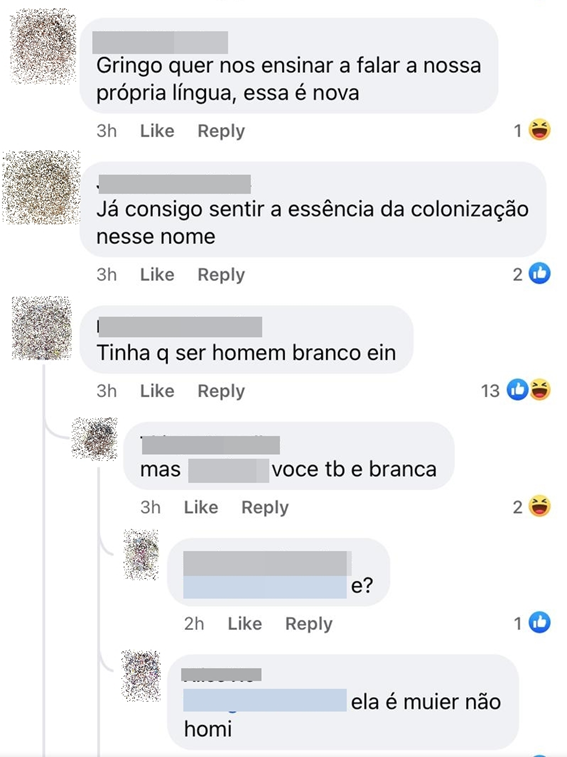
\includegraphics[width=0.85\textwidth]{Fig4.png}
 \caption{Seção de comentários 2 da Greengo Dictionary.}
 \label{fig4}
 \source{GREENGO DICTIONARY, Facebook \url{https://www.facebook.com/greengodictionary}. Acesso em: 10 de set. de 2021.}
\end{figure}

Os sujeitos que interagem nos comentários (\Cref{fig4}) acreditavam que estavam lidando com um caso de um estrangeiro/gringo que se propunha a ensinar os brasileiros a como escrever corretamente, o que pode ser inferido pelos enunciados: “Gringo quer nos ensinar a falar a nossa própria língua” e “Já sinto o cheiro da colonização nesse nome”, que ilustram também uma associação entre nacionalidade e aparência com base em estereótipos (nome “estrangeiro”). Tais relações são construídas através de dois processos: o de distinção, uma vez que a aparência e o nome de “gringo” atribuem ao Sujeito C posições identitárias que os distinguiria dos brasileiros, e do posicionamento de terceira ordem, já que o Sujeito C não faz parte da interação que se desenvolve entre os demais.  

Associado à relação de distinção, constrói-se também um posicionamento de enfrentamento aos enunciados do Sujeito C. A partir da relação de deslegitimação, quem se posiciona contrariamente assim o faz por não conferir àquele possível “gringo” a autoridade para opinar sobre uma língua que não era a sua, atribuindo a si a posse da língua portuguesa, como indicado em “a nossa própria língua”. Desse modo, as relações e posicionamentos identitários apontam para uma complexa associação entre língua, identidade e território, traduzida em termos de tríade herderiana \cite{canagarajah_translingual_2013}. Conforme tal pressuposto, tem-se uma ideologia embasada na concepção de que haveria donos legítimos de uma língua e de que ela seria um dos mecanismos para se reivindicar identidades e territórios nacionais específicos.

Já nos enunciados seguintes, são negociadas outras relações identitárias com base na atribuição de diferentes posições discursivas. O Sujeito D se posiciona comentando “Tinha q ser homem branco ein”, indicando uma ideologia linguística mais centrada em questões de gênero do que de nacionalidade. Em contrapartida, o Sujeito E, a partir de um posicionamento de primeira ordem, contesta o Sujeito D ao enunciar “mas você tb e branca”, enquadrando-a na mesma categoria identitária do Sujeito C, isto é, a de sujeitos brancos. Em sua réplica, através de um posicionamento de segunda ordem, o Sujeito D enuncia “e?”, para contestar o posicionamento atribuído e indicar que a sua crítica estava embasada no fato do Sujeito C ser homem, o que é reforçado pelo Sujeito F: “ela é muier não homi”. Com a sequência de enunciados assinalados acima, é possível observar o desenvolvimento de diferentes relações identitárias entre os sujeitos. Ao desafiar o enquadramento do Sujeito E “mas voce tb e branca”, o Sujeito D estabelece uma relação de desnaturalização. Para \textcite{bucholtz_language_2004}, essa relação é mobilizada como uma estratégia de desestabilização de essencialismos identitários. Nesse sentido, o Sujeito D frustra as expectativas do Sujeito E por se posicionar contrariamente ao Sujeito C, mesmo sendo branca. Para esse posicionamento, Sujeitos D e F evocam a identidade de “mulher” como categoria diferenciadora, sendo ela vital para a avaliação da publicação do Sujeito C. Aqui, tal posição é manipulada para marcar uma separação entre os sujeitos, seus gêneros e ideologias.

Por último, trazemos outra postagem (\Cref{fig5}) para análise com intuito de observarmos as construções identitárias e posicionamentos realizados também por meio da translinguagem.

Postagem 3

\begin{figure}[htbp]
 \centering
 
\includegraphics[width=0.65\textwidth]{Fig5.png}
 \caption{Postagem 3 da Greengo Dictionary.}
 \label{fig5}
 \source{GREENGO DICTIONARY, Facebook \url{https://www.facebook.com/greengodictionary}. Acesso em: 10 de set. de 2021.}
\end{figure}

Na \Cref{fig5}, a postagem do Sujeito G indica uma crítica ao uso de palavras estrangeiras no dia a dia. Os chamados estrangeirismos, (aqui ilustrados pelas expressões: \textit{Could you send me the} (“Poderia me enviar o”), \textit{for tomorrow} (“para amanhã”), \textit{My} (“Meu”), \textit{is next monday} (“é na próxima segunda”)) muito utilizados em diferentes esferas de comunicação, entre elas, a empresarial, têm sido tema de debate há algum tempo. A polêmica em torno do assunto é grande e foi reacendida pelo projeto de lei 1676/1999, do então deputado Aldo Rabelo, que buscava a “promoção, proteção e defesa do uso da língua portuguesa” \cite{faraco_estrangeirismos:_2011}. Reações contrárias ao projeto não demoraram a aparecer. Segundo \textcite{faraco_estrangeirismos:_2011}, a concepção de língua que parecia fundamentar a visão do deputado foi definida como “equivocada”. Já para \textcite[p. 15]{garcez_estrangeirismos:_2001}, projetos como esses trazem à tona o debate “[...] sobre o uso prestigioso e ‘correto’ da língua da comunidade e sobre a própria vida social da linguagem [...]”.

O Sujeito G aparenta retomar a polêmica do estrangeirismo ao se posicionar publicamente, de maneira bem-humorada e socialmente orientada. Com isso, ele performa, ao mesmo tempo, a identidade de sujeito autêntico e distinto, pois não só busca se distinguir dos grupos de empresários que utilizam o inglês para se comunicar, mas, ao se valer da translinguagem para construir o sentido proposto, cria um senso de pertencimento à Greengo Dictionary.			

Na seção de comentários, é possível perceber que outros sujeitos revelam suas ideologias linguísticas ao se posicionarem de forma favorável ou contrariamente à prática. Sobre isso, é pertinente evocar \textcite{garcez_estrangeirismos:_2001} mais uma vez, quando afirmam que dependendo da comunidade em que tais empréstimos (estrangeirismos) são feitos, os valores associados a eles podem ser conflitantes, apontando para diferentes ideologias linguísticas. Para discutirmos mais esse ponto, trazemos as \Cref{fig6} e \Cref{fig7}.

\begin{figure}[htbp]
 \centering
 
\includegraphics[width=0.65\textwidth]{Fig6.png}
 \caption{Seção de comentários 3 da Greengo Dictionary.}
 \label{fig6}
 \source{GREENGO DICTIONARY, Facebook \url{https://www.facebook.com/greengodictionary}. Acesso em: 10 de set. de 2021.}
\end{figure}

Com essa publicação, podemos inferir que o Sujeito H se alinha ao grupo que é favorável à incorporação de palavras estrangeiras na língua portuguesa. Ao enunciar, ele negocia posicionamentos de autenticidade, o que pode ser sugerido através do trecho “Não é para parecer chic (sic). É para ser mais eficaz a longo prazo também e globalizar aquele seguimento”, que indica também sua visão de língua inglesa ligada ao papel que ela possivelmente exerce na comunicação global. Tal ideologia linguística atribui ao inglês o status de língua da globalização, da inclusão, ou de língua franca \cite{seidlhofer_understanding_2011}, sendo essa um requisito, nos termos do sujeito, para uma melhor preparação do profissional “além do mercado local”. Ademais, o Sujeito H performa posicionamentos identitários que o associam como membro autêntico do grupo de empresários que adotam estrangeirismos, o que fica sugerido no emprego dos itens lexicais “lidamos” (nós, empresários) e das palavras inglesas \textit{casting} (“processo seletivo”) e \textit{job} (“emprego/trabalho”).	

No enunciado seguinte, o Sujeito I faz sua réplica ao comentário do Sujeito H, não para concordar ou discordar do seu posicionamento, mas para deslegitimar sua prática com base na sua própria concepção de qual seria o objetivo da página Greengo Dictionary. Ao enunciar “É só uma página que posta coisas para rirmos”, o Sujeito se posiciona como usuário autêntico da página e busca se diferenciar do posicionamento anterior. Para I, a página está voltada para diversão e não para problematizações como aquela feita pelo Sujeito G. Assim, o Sujeito I negocia a relação de deslegitimação, ao atribuir ao Sujeito H a posição de não pertencente à Greengo Dictionary, por ele não ter adotado as normas esperadas para aquele espaço de interação. Além disso, observamos também a relação de desnaturalização, uma vez que o sujeito desestabiliza a noção de pertencimento, ao considerar o posicionamento do Sujeito H como insatisfatório para os padrões locais; nesse caso, fora dos padrões da página, que teria como intuito postar coisas para rir e não para proferir “palestras”. No último comentário, também é apresentado um posicionamento contrário àquele almejado pelo Sujeito H, mas, dessa vez, centrado na (in)validação do uso de estrangeirismos, como mostramos na sequência.

\begin{figure}[htbp]
 \centering
 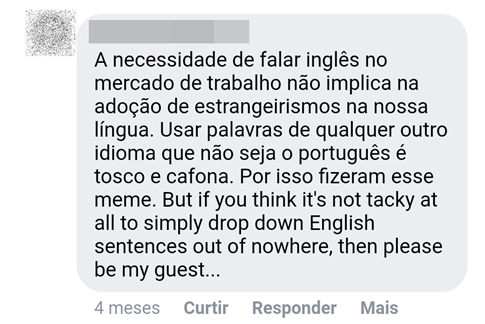
\includegraphics[width=0.85\textwidth]{Fig7.png}
 \caption{Seção de comentários 4 da Greengo Dictionary.}
 \label{fig7}
 \source{GREENGO DICTIONARY, Facebook \url{https://www.facebook.com/greengodictionary}. Acesso em: 10 de set. de 2021.}
\end{figure}

Aqui, trazemos um comentário realizado pelo Sujeito J, a partir do qual podemos depreender um posicionamento contrário à utilização de palavras estrangeiras no português: “Falar inglês no mercado de trabalho não implica na adoção de estrangeirismo na nossa língua”. Com base na análise de seus posicionamentos, observamos que as táticas intersubjetivas negociadas no discurso do Sujeito J são: de autenticidade, porque ele se autoposiciona como falante autêntico da língua portuguesa quando enuncia “nossa língua”; de distinção, quando marca discursivamente o “outro” em “qualquer outro idioma que não seja o português”; e de autoridade, quando assume o posicionamento de quem tem poder para legitimar um bom uso da língua portuguesa, embasado na ideologia de que, em interações entre brasileiros, só se pode falar ou escrever em português.				

Outra relação identitária construída nos enunciados do Sujeito J é alcançada por meio da prática translíngue. O enunciado “\textit{But if you think it’s not tacky at all to simply drop down English sentences out of nowhere, then please be my guest}” (“Mas se você acha que não é nada cafona simplesmente jogar sentenças em inglês, do nada, então, por favor, fique à vontade”), confere um “tom” irônico ao seu comentário por meio da mescla de recursos linguísticos que ele próprio critica. Com isso, o Sujeito J também se posiciona como um usuário autêntico da Greengo Dictionary, já que se valer da translinguagem atribui a ele pertencimento não somente a essa página, mas também à comunidade de sujeitos que transitam entre línguas. Dessa maneira, contraditoriamente, por meio de enunciados híbridos e embasado numa visão de “língua pura”, o Sujeito J performa diferentes posicionamentos, indexando não só o seu pertencimento à Greengo Dictionary e à comunidade de falantes de língua portuguesa, mas também a sua desaprovação ao uso de estrangeirismos e ao posicionamento do Sujeito H.

\subsection{Discussão}\label{sec-formato}
Para a análise de dados, nos embasamos na concepção de identidade como intersubjetivamente construída por meio de uma gama de posicionamentos, muitas vezes sobrepostos, que indicam relações de similaridade e diferença, genuinidade e artificialidade, e autoridade e ilegitimidade. Chamamos atenção, assim, para o caráter relacional das identidades \cite{bucholtz_identity_2005}, o que nos permitiu investigar as posições discursivas assumidas e negociadas entre sujeitos em uma página \textit{online}. Foi possível problematizar, a partir das postagens aqui discutidas, como a negociação de relações identitárias entre diferentes sujeitos está atrelada aos seus mais diversos propósitos comunicativos. Tais relações se materializam nos recursos multimodais empregados para atribuir, negar e resistir a posicionamentos no discurso. Nesse cenário, o engajamento em práticas translíngues \cite{canagarajah_translingual_2013} se mostrou preponderante não só para a construção de um sentimento de pertencimento à comunidade discursiva ora analisada, mas também para a consideração das mais diferentes ideologias linguísticas que embasam as performances identitárias dos sujeitos.			

Logo, observamos que estudar tais práticas sob uma ótica translíngue ou transidiomática \cite{moita_lopes_ideologia_2013} pode nos oferecer argumentos para indicar que, embora os sujeitos revelem ideologias ainda calcadas na ideia de uso “correto” e “puro” das línguas, seus enunciados se deslocam por meio da imbricação do português com o inglês, ressaltando não só a contradição que marca seus posicionamentos, mas também colocando em evidência a noção de língua como recurso comunicativo, que leva a efeito “[...] propósitos específicos locais situados em um mundo em que a movimentação das pessoas requer a compreensão da mobilidade de recursos linguísticos e sociolinguísticos [...]”. \cite[p. 113]{moita_lopes_ideologia_2013}. 	

Ao buscarmos caminhos analíticos que pudessem fazer jus tanto à noção de identidade como prática discursiva quanto aos mais diferentes processos de negociação identitária, confrontamos duas propostas teórico-analíticas, quais sejam, a dos posicionamentos e das táticas de intersubjetividade. A partir delas, investigamos os modos em que as relações de adequação e distinção, autenticação e desnaturalização e autorização e deslegitimação são construídas discursivamente. Com isso, discutimos os sentidos negociados pelos sujeitos quando se autoposicionam como legítimos falantes de uma língua e com o poder de legitimar outros usos linguísticos, bem quando buscam se diferenciar de outros grupos identitários e deslegitimar suas práticas. Observamos, portanto, que a manipulação de recursos verbais e não verbais constitui uma estratégia elaborada, através da qual os sujeitos negociam posições identitárias diversas, dando pistas de suas ideologias.	Dessa maneira, avaliamos que as práticas comunicativas desenvolvidas na página Greengo Dictionary funcionam como importantes ferramentas para o alinhamento ou resistência a diferentes discursos sociais e políticos. Nesse contexto, o envolvimento em processos de hibridação representa uma das ações por meio das quais os usuários performam suas identidades e negociam sentidos possíveis sobre as línguas. Enunciar nessa comunidade significa, portanto, se envolver em diferentes posicionamentos, com sujeitos se deslocando entre concepções mais fixas e homogêneas de língua e identidade, como também de práticas mais abertas à diversidade e à mistura de recursos semióticos.


\section{Conclusão}\label{sec-modelo}
Por meio do discurso \textit{online} de usuários da Greengo Dictionary, aqui compreendida como uma comunidade discursiva do Facebook, nosso objetivo foi o de problematizar as ideologias que fundamentam os diferentes usos linguísticos nessa página. Diante disso, ao entendermos o inglês e português como línguas de fronteira, híbridas e que transitam entre diferentes perspectivas e propósitos comunicativos, foi possível investigar as ideologias linguísticas dos sujeitos, confrontando-as com concepções baseadas num possível normativismo linguístico.				

A fim de procedermos às análises das postagens e comentários selecionados para este estudo, partimos dos conceitos de posicionamento \cite{harre_positioning_1999}, posturas \cite{barton_linguagem_2015} e das táticas de intersubjetividade \cite{bucholtz_language_2004,bucholtz_identity_2005}, que nos permitiram observar que os sujeitos negociam posições identitárias com vistas à construção de diferentes relações entre eles, quais sejam, a de adequação/distinção, autenticação/desnaturalização e autorização/deslegitimação.	 			

Isso posto, acreditamos que este artigo possa ser um ponto de partida para estudos que tenham como intuito investigar a comunicação mediada pela tecnologia digital, com foco nas ideologias que fundamentam os posicionamentos identitários de membros de diferentes comunidades discursivas \textit{online}. Atrelados a isso, ressaltamos a necessidade de mais trabalhos no campo da linguagem buscarem a perspectiva dos próprios envolvidos nas práticas analisadas. Embora o escopo deste artigo não tenha contemplado tal proposta, julgamos ser relevante a abordagem êmica nesse contexto, como forma de confrontar as interpretações dos sujeitos participantes com as perspectivas teórico-metodológicas que orientam os pesquisadores em suas investigações.


\printbibliography\label{sec-bib}
% if the text is not in Portuguese, it might be necessary to use the code below instead to print the correct ABNT abbreviations [s.n.], [s.l.]
%\begin{portuguese}
%\printbibliography[title={Bibliography}]
%\end{portuguese}


%full list: conceptualization,datacuration,formalanalysis,funding,investigation,methodology,projadm,resources,software,supervision,validation,visualization,writing,review
\begin{contributors}[sec-contributors]
\authorcontribution{Bruna de Almeida Oliveira Moreira}[conceptualization,methodology,writing]
\authorcontribution{Diogo Oliveira do Espírito Santo}[conceptualization,methodology,review]
\end{contributors}

\end{document}

